\documentclass{beamer}
\usepackage{outlines}
\usepackage{amsmath}
\usepackage[T1]{fontenc}
\usepackage{amssymb}
%\newcommand\numberthis{\addtocounter{equation}{1}\tag{\theequation}}


\title{\huge Functional Data Analysis for Sparse Longitudinal Data}
\subtitle{\large Fang YAO, Hans-Georg M\"{u}LLER, and Jane-Ling WANG \\
\normalsize Journal of the American Statistical Association }
\author{Wangfei Wang}




%\usetheme{lucid}
\begin{document}
\graphicspath{{../Report/Figures/}}
	\frame {
		\titlepage
	}
	\frame{
	    \frametitle{What is the main problem the paper trying to address?}
	    \begin{outline}
	    \1 \textbf{Introduction} 

		    Functional principal components (FPC) analysis characterizes the dominant mode of variation around an overall mean trend function, and therefore is popular in longitudinal data analysis. 
	    \1 \textbf{Limitations of available models:}
	    	\2 Cannot deal with infrequent, irregularly-spaced repeated measures.
	    	\2 Some kernel-based FPC analysis [ref] cannot be approximated by the usual integration method.
	    	\2 Linear mixed models or reduced-rank mixed effects models using B-splines to model the individual curves with random coefficients [refs] are too complex, and the asymptotic properties of the estimated components were not investigated. 
	    \end{outline}
	}
	\frame{
	    \frametitle{What is the proposed solution?}
		\begin{outline}
		\1 They proposed a version of FPC analysis, in which they framed the FPC scores as conditional expectations.
		And thus they coined this method ``principal components analysis through conditional expectation (\textbf{PACE})''.
		\1 \textbf{Contributions of the paper}
			\2 In the model, they took into account the additional measurement errors. 
			\2 They derived the asymptotic consistency properties.
			\2 They derived the asymptotic distribution needed for obtaining point-wise confidence intervals for individual trajectories. 
		\end{outline}
		
	}
	\frame{
		\frametitle{Innovation}
		%\framesubtitle{An Example of Lists}
		\begin{itemize}
			\item The proposed conditional model is designed for sparse and irregular longitudinal data. 
			\item Under Gaussian assumptions, the authors showed that estimation of individual FPC scores are the best prediction; and under non-Gaussian assumption, they provide estimates for best linear prediction. 
			\item One-curve-leave-out cross-validation was proposed to choose auxiliary parameters. 
			\item Akaike information criterion (AIC) was used for faster computation to select eigenfunctions. 
		\end{itemize}
	}
	\frame{
	    \frametitle{METHOD: PACE}
	    \begin{itemize}
			\item Model with Measurement Errors 
			\item Estimation of the Model Components 
			\item Functional Principal Components Analysis Through Conditional Expectation
			\item Asymptotic Confidence Bands for Individual Trajectories
			\item Selection of the Number of Eigenfunctions
		\end{itemize}
	}
	\frame{
	    \frametitle{Methods: Model with Measurement Errors}
	    \underline{Assume:} 1) Trajectories are independent realizations of a smooth random function with unknown mean $E{X(t)} = \mu(t)$ and covariance $cov(X(s), X(t)) = G(s,t)$, where domain of X($\cdot$) is $\mathcal{T}$.

		2) G has an orthogonal expansion in terms of eigenfunction $\phi_k$ and eigenvalues $\lambda_k$: $G(s,t) = \sum_k{\lambda_k\phi_k(s)\phi_k(t)}, \; \; t, s \in \mathcal{T}$, where $\lambda_1 \geq \lambda_2 \geq \cdot \cdot \cdot$.

		\underline{Model:}
		\begin{align}
			\label{eq:eq1}
			Y_{ij} &= X_i(T_{ij}) + \epsilon_{ij}  \\
			&= \mu(T_{ij}) + \sum_{k=1}^\infty \xi_{ik}\phi_k(T_{ij}) + \epsilon_{ij}, \; \; \;  T_{ij} \in \mathcal{T} 
		\end{align}
		where $E{\epsilon_{ij}} = 0$, var($\epsilon_{ij}$) = $\sigma^2$. 

		$Y_{ij}$ is the jth observation of the random function X($\cdot$), and $\epsilon_{ij}$ is the measurement errors that are iid and are independent of random coefficients $\xi_{ik}$, where $i = 1, ..., n; j = 1, ..., N_i; k = 1, 2, ...$.
	}
	\frame{
	    \frametitle{Methods: Estimation of the Model Components}
	    \begin{itemize}
		    \item{Estimation of mean function $\mu$}

			 Minimizing the following equation \eqref{eq:A2} respect to $\beta_0$ and $\beta_1$
			
			\begin{align}
				\label{eq:A2}
				\sum_{i=1}^{n}\sum_{j=1}^{N_i}\kappa_1(\frac{T_{ij}-t}{h_\mu})\{Y_{ij}-\beta_0-\beta_1(t-T{ij})\}^2{}
			\end{align}
			where $\kappa_1$ is a kernel function: ${\rm I\!R} \rightarrow {\rm I\!R} $.

			Then estimation of mean function $\mu$ can be obtained:
			\[\hat{\mu}(t) = \hat{\beta_0}(t)\]
			\end{itemize}
	}
	\frame{
	    \frametitle{Methods: Estimation of the Model Components}
	    \begin{itemize}
			\item{Estimation of measurement errors $\sigma^2$}
			\begin{align}
			    \label{eq:eq2}
			    \hat{\sigma^2} &= \frac{2}{|\mathcal{T}|}\int_{\mathcal{T}_1}\{\hat{V}(t) - \tilde{G}(t)\}dt 
			\end{align}
			if $\hat{\sigma}^2>0$ and $\hat{\sigma}^2 = 0$ otherwise.

			where $|\mathcal{T}|$ is the length of $\mathcal{T}$, $\mathcal{T_1} = [inf\{x: x \in \mathcal{T}\} + |\mathcal{T}|/4]$,

			$\tilde{G}$ is the diagonal of the surface estimate

			$\hat{V}(t)$ is a local linear smoother focusing on diagonal values $\{G(t,t) + \sigma^2\}$.

			\vspace{3mm}
			Estimation procedures for $\tilde{G}$: 

			$\hat{G}(s,t) \rightarrow$ surface estimate $\bar{G}(s,t) \rightarrow \tilde{G}(t) = \bar{G}(0, t/\sqrt(2))$, where $G(s, t)$ is the ``raw covariance'' $cov(X(s), X(t))$.
		\end{itemize}
	}
	\frame{
	    \frametitle{Methods: Estimation of the Model Components}
	    \begin{itemize}
		    \item{Estimation of eigenfunctions and eigenvalues $\phi_k$ and $\lambda_k$}

		    Solutions $\phi_k$ and $\lambda_k$ of the following eigenequation:
			\begin{align}
				\label{eq:eq3}
				\int_\mathcal{T} \hat{G}(s,t)\hat{{\phi_k}}(s)ds &= \hat{\lambda_k}\hat{\phi}_k(t)
			\end{align}
			where the $\hat{\phi}_k$ are subject to $\int_\mathcal{T}\hat{\phi}_k(t)^2dt = 1$ and $\int_\mathcal{T}\hat{\phi}_k(t) \times \hat{\phi}_m(t)dt = 0$ for $m<k$.
		\end{itemize}
	}
	\frame{
	    \frametitle{Methods: Functional Principal Components Analysis Through Conditional Expectation}
	    \begin{itemize}
			\item Under the assumption that $\xi_{ik}$ and $\epsilon_{ij}$ are jointly Gaussian:
			\begin{align}
				\label{eq:eq5}
				\hat{\xi}_{ik} = \widehat{E}{[\xi_{ik}|\widetilde{\pmb{Y}}_i]} = \hat{\lambda}_k\hat{\pmb{\phi}}_{ik}^T\hat{\pmb{\Sigma}}_{\pmb{Y}_i}^{-1}(\tilde{\pmb{Y}}_i - \hat{\pmb{\mu}}_i)
			\end{align}
			where $(\hat{\pmb{\Sigma}}_{\pmb{Y}_i})_{j,l} = \hat{G}(T_{ij}, T_{il}) + \sigma^2\delta_{jl}$ is the $(j,l)$th element of $\hat{\pmb{\Sigma}}_{\pmb{Y}_i}$. 
			Under the Gaussian assumption, the $\tilde{\xi}_{ik} = E[\xi_{ik}|\widetilde{\pmb{Y}}_i]$ is the best prediction of the FPC score. 
			\item The prediction for the trajectory $X_i(t)$ for the $i$th subject using the first K eigenfunctions is then:
			\begin{align}
				\label{eq:eq6}
				\widehat{X_i}^K(t) = \hat{\mu}(t)+\sum_{k=1}^{K}\hat{\hat{\xi}}_{ik}\hat{\phi}_k(t)
			\end{align}
			\item In simulation result, the authors showed that this proposed model is also robust when the Gaussian assumption does not hold. 
		\end{itemize}

	}
	\frame{
	    \frametitle{Methods: Asymptotic Confidence Bands for Individual Trajectories}
	    \begin{itemize}
		    \item The $(1-\alpha)$ asymptotic simultaneous confidence bands for $X_i(t)$ can be obtained:
			\begin{align}
				\label{eq:eq8}
				\widehat{X}_i^K(t) \pm \sqrt{\chi^2_{K,1-\alpha}\hat{\pmb{\phi}}_{K,t}^T\widehat{\pmb{\Omega}}_K\hat{\pmb{\phi}}_{K,t}}
			\end{align}
			where $\chi^2_{K,1-\alpha}$ is the $100(1-\alpha)$th percentile of the chi-squared distribution with K degrees of freedom. 

			\item For all linear combinations of the FPC scores, the authors proved that they could be obtained by:
			\begin{align}
				\label{eq:eq9}
				\pmb{I}^T\pmb{\xi}_{K,i} \in \pmb{I}^T\hat{\pmb{\xi}}_{K,i} \pm \sqrt{\chi^2_{d,1-\alpha}\pmb{I}^T\widehat{\pmb{\Omega}}\pmb{I}}
			\end{align}
			with approximate probability $(1-\alpha)$, where $\mathbf{I}\in \mathcal{A}$, $\mathcal{A} \subseteq {\rm I\!R}^K$ is a linear space with dimension $d\leq K$.
		\end{itemize}
	}
	\frame{
		\frametitle{Methods: Selection of the Number of Eigenfunctions}
		\begin{itemize}
			\item Choose the number of eigenfunctions K that minimizes the cross-validation score:
			\begin{align}
				\label{eq:eq10}
				CV(K) = \sum_{i=1}^{n}\sum_{j=1}^{N_i}\{Y_{ij}-\widehat{Y}_i^{(-i)}(T_{ij})\}^2
			\end{align} 
			where $\widehat{Y}_i^{(-i)}(t) = \hat{\mu}^{(-i)}(t) + \sum_{k=1}^{K}\hat{\xi_{ik}}^{(-i)}(t)\hat{\phi}_{k}^{(-i)}(t)$. 
			%, where $\hat{\xi}_{ik}$ can be obtained from \eqref{eq:eq5}.

			\item AIC-type criteria was found to be more computationally efficient. 
			A pseudo-Gausian log-likelihood was generated:
			\begin{flalign}
			&\begin{aligned}
				& \widehat{L} = \sum_{i=1}^n\big\{-\frac{N_i}{2}log(2\pi) - \frac{N_i}{2}log\hat{\sigma}^2 -  \\ 
				&\frac{1}{2\hat{\sigma}^2}(\widetilde{\pmb{Y}}_i - \hat{\pmb{\mu}}_i - \sum_{k=1}^{K}\hat{\xi}_{ik}\hat{\pmb{\phi}}_{ik})^T \times (\widetilde{\pmb{Y}}_i - \hat{\pmb{\mu}}_i - \sum_{k=1}^{K}\hat{\xi}_{ik}\hat{\pmb{\phi}}_{ik}) \big\} \label{eq:eq11}
			\end{aligned}&&
			\end{flalign}
			where AIC = $-\widehat{L} + K$.
		\end{itemize}
	}
	\frame{
	    \frametitle{Asymptotic Properties}
	   	\begin{itemize}
		   	\item $\underset{t \in \mathcal{T}}{sup}|\hat{\mu}(t) - \mu(t)| = O_p \left(\frac{1}{\sqrt{n}h_{\mu}} \right)$ 
		   	\item $\underset{{t,s} \in \mathcal{T}}{sup}|\hat{G}(s,t) - G(s,t)| = O_p \left(\frac{1}{\sqrt{n}h_{G}^2} \right), |\hat{\lambda}_k - \lambda_k| = O_p \left(\frac{1}{\sqrt{n}h_{G}^2} \right) $, 
		   	$||\hat{\phi}_k - \phi_k||_H = O_p \left(\frac{1}{\sqrt{n}h_{G}^2} \right), k \in \mathcal{T}^{'}$
		   	\item $\underset{{t} \in \mathcal{T}}{sup}|\hat{\phi_k}(t) - \phi_k(t)| = O_p \left(\frac{1}{\sqrt{n}h_{G}^2} \right), k \in \mathcal{T}^{'}$ 
		   	\item $\underset{n \rightarrow \infty}{lim} \hat{\xi}_{ik} = \tilde{\xi}_{ik}, \underset{K \rightarrow \infty}{lim}\underset{n \rightarrow \infty}{lim} \widehat{X}_i^K(t) = \widetilde{X}_i(t) \; \; \forall t \in \mathcal{T}$ in probability. 
			\item $\underset{K \rightarrow \infty}{lim}\underset{n \rightarrow \infty}{lim} P\left\{\frac{\widehat{X}_i^K(t) - X_i(t)}{\sqrt{\omega_K(t,t)}} \leq x \right\} = \Phi(x) $, where $\Phi(x) $ is the standard Gaussian cdf.
			\item $\underset{n \rightarrow \infty}{lim} P\left\{ \underset{t \in \mathcal{T}}{sup} \frac{|\widehat{X}_i^K(t) - X_i^K(t)|}{\sqrt{\omega_K(t,t)}} \leq \sqrt{\chi_{K, 1-\alpha}^2} \right \} \geq 1-\alpha $, where $\chi_{K, 1-\alpha}^2$ is the $1-\alpha$th percentile of the chi-squared distribution with K degrees of freedom. 
		\end{itemize}
	}
	\frame{
	    \frametitle{Simulation Studies}
	    \begin{figure}[h]
			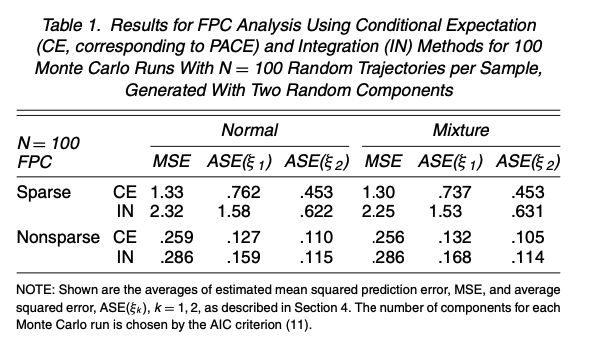
\includegraphics[width = 4 in]{Table1.png}
			\centering
		\end{figure}
		\[MSE = \sum_{i = 1}^{n} \int_{0}^{10} \left\{X_i(t) - \widehat{X}_i^K(t) \right\}^2 dt/n \]
		\[ASE(\xi_k) = \sum_{i = 1}^n (\hat{\xi}_{ik} - \xi_{ik})^2/n \; \; k = 1, 2.\] 
	}
	\frame{
	    \frametitle{Applications}
	    \begin{itemize}
	    	\item Longitudinal CD4 Counts
	    	\item Yeast Cell Cycle Gene Expression Profiles
	    \end{itemize}
	}
	\frame{
	    \frametitle{Potential applications of the proposed method}
	    This is a paragraph.
	}
	\frame{
	    \frametitle{Propose one or two possible topics/questions for future research in this area.}
	    This is a paragraph.
	}
	\frame{
	    \frametitle{Paragraph Content}
	    This is a paragraph.
	}
	\frame{
	    \frametitle{Paragraph Content}
	    This is a paragraph.
	}
	\frame{
	    \frametitle{Paragraph Content}
	    This is a paragraph.
	}
	\frame{
	    \frametitle{Paragraph Content}
	    This is a paragraph.
	}
	\frame{
	    \frametitle{Paragraph Content}
	    This is a paragraph.
	}
	\frame{
	    \frametitle{Paragraph Content}
	    This is a paragraph.
	}
	\frame{
	    \frametitle{Paragraph Content}
	    This is a paragraph.
	}
	\frame{
	    \frametitle{Paragraph Content}
	    This is a paragraph.
	}
	\frame{
	    \frametitle{Paragraph Content}
	    This is a paragraph.
	}
	\frame{
	    \frametitle{Paragraph Content}
	    This is a paragraph.
	}
	\frame{
	    \frametitle{Paragraph Content}
	    This is a paragraph.
	}
	\frame{
	    \frametitle{Paragraph Content}
	    This is a paragraph.
	}
\end{document}